% Report file. 

% Preamble.
%{{{

\documentclass[a4paper,oneside,11pt]{article}

\usepackage[margin=2cm]{geometry}
\usepackage{parskip}

\usepackage{helvet}
\renewcommand{\familydefault}{\sfdefault}

\usepackage{amsmath}

\usepackage{xcolor}

\usepackage{listings}
\lstset{
	basicstyle=\ttfamily\footnotesize,
	numbers=left,
	showstringspaces=false,
	commentstyle=\itshape\color{green!50!black},
    	keywordstyle=\color{orange},
	identifierstyle=\color{blue},
    	stringstyle=\color{red!75!black},
}

\usepackage{graphicx}
\graphicspath{ {./images} }

\usepackage{tikz}

\usepackage{url}
\usepackage{hyperref}
\hypersetup{
	colorlinks=true,
	linkcolor=black,
	citecolor=red,
	urlcolor=blue
}

\usepackage{pgfgantt}

\usepackage[firstinits=true,style=trad-abbrv]{biblatex}
\addbibresource{bibliography.bib}

\begin{document}

%}}}

% Title page and abstract.
%{{{

\title{Machine Learning for Side Channel Attacks}
\author{Literature Review and Project Specification}
\date{}

\maketitle

\textbf{Abstract:} The rise of fledgling technologies such as cloud computing
and the Internet of Things and the proliferation of cryptographic algorithms
and protocols has raised concerns around the security of these; notably that
side channel attacks would be particularly effective against poorly implemented
cryptography, potentially affecting a myriad of systems. Side channel attacks
are a class of attacks where a third party can extract extra information and
secrets from the implementation details of an algorithm or protocol, as opposed
to finding flaws in the algorithm itself (as is the case in traditional
cryptanalysis). Examples include timing and power monitoring attacks against
cryptosystems, many of which have been shown to be effective in a variety of
contexts and environments. Machine learning is the process of using computers
to learn from data, and has strong applications to side channel attacks for
automating analysis and increasing effectiveness compared with previous
techniques. This paper covers the uses of machine learning in side channel
attacks against cryptosystems and proposes a project to demonstrate their
efficacy.

\vspace*{\fill}

\begin{center}
	\textit{I certify that all material in this dissertation which is not
	my own work has been identified.}
\end{center}

\thispagestyle{empty}
\setcounter{page}{0}

\newpage

%}}}

% Introduction.
%{{{

\section{Introduction and Motivation}
\label{sec:introduction-and-motivation}

The rapid expansion of the internet, in terms of users, devices and
applications, has led to the necessary adoption of modern cryptography:
understanding how data can be securely transmitted such that only the intended
recipient(s) can understand the information being sent
\cite{B/Introduction-Cryptography}. This field is essential to ensuring that
communications over untrusted networks (such as the internet) are secure and
trustworthy, and a significant portion of research is dedicated to analysing
cryptographic systems and algorithms to discover how they can be broken. The
intention is to understand their flaws and weaknesses, and use these to design
systems which offer better security and are more effective; the use of
offensive techniques to evaluate security is commonplace in the field of
computer security and is considered best practice to ensure that an attacker
cannot violate the confidentiality, integrity or authenticity of a system.

Side channel attacks (SCAs) refer to a class of attacks which focus on finding
flaws in the implementation details of an algorithm or protocol, which may leak
extra information about the computation being performed
\cite{B/Secure-ICs-Systems}. Examples of side channels which can be leveraged
to attack a computer system include timing and execution speed, cache
hits/misses, power consumption, electromagnetic radiation (such as light, radio
waves and microwaves), and acoustic information (such as sound and vibration).
SCAs can be used in conjunction with cryptanalysis and software security
testing to uncover flaws in modern computer systems which may not be found
using traditional techniques. A well known example of such flaws are the
Spectre and Meltdown CPU bugs \cite{A/Lipp-2020-Meltdown,
A/Kocher-2020-Spectre}, which were discovered using cache and timing attacks,
and allow a process to read all memory. As of 2018, these vulnerabilities
affect nearly every computer in the world \cite{W/Meltdown-and-Spectre}.

Machine learning (ML) is the study of how computers can find patterns in data
and learn to perform tasks automatically without being explicitly programmed to
do so \cite{B/Automated-Design-Genetic-Programming}. Typical machine learning
tasks include: predicting values (either discrete or continuous) for some
unseen data based on a previous dataset with labelled values (supervised
learning \cite{B/Foundations-of-Machine-Learning}); identifying patterns or
``clusters" within a dataset without being given any information a priori
(unsupervised learning \cite{B/Elements-Statistical-Learning}); and finding
optimal behaviours or routines to maximise some reward in an environment
(reinforcement learning \cite{B/Reinforcement-Learning}). ML has applications
in a wide variety of fields, including medicine, computer vision, email
filtering and large language modelling, and is highly useful where an
analytical algorithm may be too costly to develop or may not exist at all.
Machine learning also strong applications to security, in particular to side
channel attacks, and often results in attacks which are more effective than
their non-ML counterparts, as shown later in the literature review.

The motivation of this paper is to understand how machine learning can be
applied to side channel attacks to make them more effective in comparison with
traditional techniques. While several non-ML approaches currently exist for
different classes of SCAs (e.g., template attacks for power analysis, etc.),
these are difficult to implement and often require a large amount of effort
with diminishing returns. Furthermore, the typical workflow for carrying out
these attacks -- collecting a large number of sample observations and using
analysis to discover secrets -- naturally lends itself to ML techniques.
Lastly, the diversity of algorithms, protocols, devices and platforms that
currently exist is of concern to the security community at large: analysing and
understanding the flaws which may exist in all of these is a significant, if
not impossible undertaking. Emerging technologies such as the Internet of
Things and cloud computing have exacerbated these fears, and consequently it is
necessary to find approaches for discovering vulnerabilities which are
effective and efficient. This paper proposes a project to demonstrate the
efficacy of machine learning for side channel attacks, and discover new attacks
on existing cryptographic systems.

%}}}

% Literature Review.
%{{{

\section{Literature Review}
\label{sec:literature-review}

This section covers the background material of this paper necessary to
understand the concepts discussed and the project proposed, including a survey
of research being conducted in this area.

% Introduction to SCAs.
%{{{

\subsection{Introduction to Side Channel Attacks}
\label{sec:introduction-to-scas}

As described previously, side channel attacks refer to attacks which exploit
information leakage across side channels (such as timing/execution speed, power
consumption, etc.) which are not typically considered when implementing an
algorithm or protocol. These side channels can be used to deduce secret
information in a system, as described in table \ref{tbl:sca-descriptions}.

\begin{table}[h]
	\centering
	\footnotesize

	\begin{tabular}{|l|p{10cm}|}
		\hline
		\textbf{Side Channel Attack} & \textbf{Description} \\
		\hline
		Timing Attacks & Attacks focused on measuring the execution
		times of a computation. \\
		\hline
		Cache Attacks & Attacks which monitor the cache of a computer
		and use this to infer secret information based on cache hits
		and misses. \\
		\hline
		Power Monitoring Attacks & Attacks which monitor the power
		consumption of a device during certain operations and uses
		power traces to deduce secrets. \\
		\hline
		Electromagnetic Attacks & Attacks which measure the radio waves
		and/or microwaves emitted from a device during computation and
		can often directly lift plain text data from secure devices. \\
		\hline
		Optical Attacks & Attacks which monitor the activity of a
		computer using video recording and uses this information to
		find secrets. \\
		\hline
		Acoustic Attacks & Attacks which correlate fan speed/noise and
		low frequency noise emitted by the CPU with power consumption,
		and uses audio recordings to guess secrets. \\
		\hline
		Fault Attacks & Attacks which deliberately introduce faults
		into a system to evaluate the current internal state. \\
		\hline
	\end{tabular}

	\caption{Side channel attacks and their descriptions.}
	\label{tbl:sca-descriptions}
\end{table}

Side channel attacks can vary by their application, environment and
requirements. Some SCAs can be performed as black-box attacks against unknown
systems, while others require deeper knowledge about the system being attacked
including the algorithm or protocol being used and technical details around the
implementation of these. Furthermore, some SCAs are only effective when the
attack has physical access to the system (as is the case with power monitoring,
electromagnetic and acoustic attacks) while others can take place on remotely,
over multiple networks and even across the internet (such as timing and cache
attacks). Finally, different side channels will require unique approaches to
actually perform the attack. Nonetheless, they all follow the same basic
process:

\begin{enumerate}
	\item{Gather a (potentially large) number of sample observations,
		usually based on some input.}
	\item{Perform analysis on the results to (sometimes partially) infer
		secret information.}
	\item{Repeat the previous steps till the secret is completely
		discovered, usually adjusting the input according to the
		results.}
\end{enumerate}

It should be noted that side channel attacks differ from traditional
cryptanalysis and software security testing. Cryptanalysis focuses on the
mathematical aspect of security and cryptography, using techniques such as
model checking and cryptographic attacks to analyse the security of algorithms
and protocols. Software security testing examines a system to discover flaws
which an attacker can exploit to breach its security, with prime examples
including SQL injections and buffer overflow attacks. Side channel attacks
instead focus on how an algorithm or protocol can leak information across
external channels which are not generally considered during cryptanalysis or
security testing but still pose a significant threat. Nonetheless, it is used
in conjunction with these fields to ensure security in computer systems, and
eliminate potential attack vectors which malicious third parties can exploit.
It should also be noted that extracting secrets by analysing and influencing
human behaviour is not considered a side channel attack -- this falls under
social engineering.

SCAs are of particular concern to researchers as they are typically more
fruitful and easier to implement compared with traditional cryptanalysis and
consider attack vectors which are not usually taken into account with security
testing. Furthermore, given the widespread use and reliance on cryptography, it
is paramount that these kinds of flaws are identified so they can be
eliminated. Current research suggests that modern web applications
\cite{A/Chen-2010-SCA-Web}, mobile and IoT devices \cite{A/Lyu-2018-SCA-IoT},
cloud systems \cite{A/Bazm-2017-SCA-Cloud} and cryptographic systems in general
\cite{A/Zhou-2005-SCA-Cryptography} are at high risk of being vulnerable to
side channel attacks, with cryptographic failures being the second highest
vulnerability listed as part of the OWASP Top 10 for 2021
\cite{W/OWASP-Top-10}. It is therefore necessary to develop techniques for
efficiently identifying if a particular device or system is vulnerable to a
side channel attack or not.

This paper focuses on timing and monitoring attacks as examples of SCAs which
could have machine learning applied to them.

%}}}

% Timing attacks.
%{{{

\subsection{Timing Attacks}
\label{sec:timing-attacks}

In a timing attack, the attacker measures the amount of time it takes for an
algorithm to complete execution \cite{A/Kocher-1996-Timing}. Each operation on
a computer takes a certain amount of time to execute, and the amount of time
may vary depending on the input. An attacker can examine the times taken for a
particular operation to be performed with different inputs and use this
information to deduce a secret, for example the password of a user. Consider
the Python program given in figure \ref{src:str-comp-function}:

\begin{figure}[h]
	\begin{lstlisting}[language=Python]
# Compare 2 strings. Return True if they
# are the same and False if not.
def compare_strings(str_1, str_2):
    if len(str_1) != len(str_2):    # Compare string lengths.
    	return False

    str_length = len(str_1)
    for i in range(str_length):     # Iterate through each character.
	if str_1[i] != str_2[i]:    # Compare individual characters.
	    return False

    return True

secret_string = "0123456789"

# Operation 1:
compare_strings(secret_string, "abcdefghij")

# Operation 2:
compare_strings(secret_string, "012345678X")
	\end{lstlisting}

	\caption{An insecure string comparison function.}
	\label{src:str-comp-function}
\end{figure}

The function terminates much quicker in the first operation compared with the
second, due to the linear manner in which comparisons are made. An adversary
can supply this function with multiple strings and compare the execution times
for each, and use this information to deduce what the value of
\texttt{secret\_string} is. This attack can be extended to more complicated
operations, provided that timing variations for execution are dependent on the
input given to the algorithm. External noise (such as network traffic or CPU
scheduling) can cause the attack to be slightly more difficult, however
statistical correlation analysis can be performed to fully recover the value of
a secret. This attack is powerful as it is simple to understand and implement
and has low computational demands, but requires knowing the internal
mechanisms of the algorithm implementation being attacked to understand where
data-dependent timing variations can be introduced.

In 1996, Kocher presented a timing attack against RSA and Diffie-Hellman along
with several other cryptographic schemes \cite{A/Kocher-1996-Timing}. This
attack was the first of its kind, and demonstrated that an attacker could
factor RSA keys, discover exponents for Diffie-Hellman, etc., without
performing complicated mathematics or brute force attacks, which are extremely
difficult and expensive operations to carry out. Kocher stresses that while the
attack is computationally efficient, it is also highly dependent on the details
around the implementation of an algorithm: in Kocker's case, the
square-and-multiply algorithm used for modular exponentiation introduces timing
variations depending on the input parameters.

Kocher describes the following scenario: an attacker is attempting to guess
some secret \( s \) which is used with some algorithm implementation \( P \) to
perform some cryptographic computation (e.g. decryption, digital signing, etc.)
on some input \( m \). It is given that \( M \) is the set of possible inputs
and \( S \) is the set of possible secrets. Additionally, attacker knows the
following functions:\\
\( P: M \times S \to \theta: (m, s) \to P(m, s) \), the implementation of the
algorithm.\\
\( T: M \times S \to \tau: (m, s) \to T(m, s) \), the time taken for \( P(m, s)
\) to be computed.

Given that the attacker has already guessed the first \( i - 1 \) bits of \( s
\), the attacker can construct two messages \( m_0 \) and \( m_1 \) where the
first bits are the correctly guessed bits and the last bit of \( m_0 \) is 0
and the last bit of \( m_1 \) is 1. The attacker can then find \( t_0 = T(m_0,
s) \) and \( t_1 = T(m_1, s) \) and, based on appropriate statistical analysis
of \( t_0 \) and \( t_1 \), accept either \( m_0 \) or \( m_1 \) as the message
containing the \( i \)th bit of \( s \). This process is repeated until the entire
secret has been recovered. This method can be trivially extended to other types
of secrets (e.g. binary strings, ciphertexts, etc.). The actual statistical
analysis will depend on the algorithm being used, the properties of the
inputs/outputs being computed, the environment the system takes place in (to
account for noise), etc. but the core principle remains the same.

As part of their research, Kocher also suggested several defence mechanisms
against this attack, including:

\begin{itemize}
	\item{Forcing all operations to run at a constant time quantum: this
		method is flawed as it does not take into account multiple
		platforms which may cause variations in timing (e.g. due to
		cache hits/misses, etc.) and unwanted compiler optimisations.}
	\item{Adding random noise to the algorithm: while feasible, defeating
		this method is simply a case of gathering more sample
		observations. In their paper, Kocher suggests that the number
		of samples required would increase from 10\textsuperscript{6}
		to 10\textsuperscript{7} -- while not feasible at the time, it
		does not provide a great amount of security assurance.}
	\item{Using blinding methods to introduce randomness to the function
		\cite{A/Chaum-1983-Blinding}: this method is generally
		preferred despite the penalty performance as it more reliable
		and introduces noise in the data being computed, rather than
		simply increasing the time of computation, meaning an attacker
		cannot accurately guess the actual secret.}
\end{itemize}

Kocher's attack, while limited in application and highly theoretical, gave rise
to several other attacks which follow the same principles. In 2005, Brumley and
Boneh demonstrated that OpenSSL's implementation of RSA was vulnerable to
timing attacks, despite using Chinese Remainder Theorem and Montgomery
Reductions to carry out the algorithm (which was previously considered
impervious to timing attacks) \cite{A/Brumley-2005-Remote-TAs}. Notably, the
attack they carried out was over a network connection, which had been thought
to be impractical due to the noise that may be introduced when transmitting
data across a network. This attack led to the widespread adoption of blinding
techniques to prevent such attacks.

Several similar attacks have been demonstrated to be highly effective against a
wide variety of algorithms, protocols, devices and systems. A practical
implementation of Kocher's attack was shown to be highly effective against the
CASCADE smart card system by Dhem et al. who were able to recover a 512 bit key
in a few hours using 300,000 sample observations and able to recover a 128 bit
key in just a few seconds using 10,000 sample observations
\cite{A/Dhem-2000-Timing-Practical}. Similar to Brumley, this work demonstrated
that timing attacks are highly practical and have real world impacts. Bernstein
showed that timing attacks were effective against AES encryption in 2005
\cite{A/Bernstein-2005-Timing-AES}, which was followed by another attack by
Bonneau and Mironov in 2006 following on from Bernstein's findings by being
able to recover a 128 bit key using only 2\textsuperscript{13} samples, an
improvement by a factor of almost four \cite{A/Bonneau-2006-Timing-AES}. These
findings led to timing attack resistant implementations of AES, first presented
by K{\"a}sper and Schwabe, which claimed to be a constant time implementation
of AES-GCM with a speed of 21.99 cycles per byte
\cite{A/Kasper-2009-Timing-AES}.  Brumley demonstrated again in 2011 OpenSSL
was still vulnerable to remote timing attacks, this time focusing on the ECDSA
algorithm \cite{A/Brumley-2011-Remote-TAs}. Timing attacks were also shown to
be effective at recovering user keystrokes and passwords from SSH sessions (as
shown by Song et al. \cite{A/Song-2001-Timing-SSH}), and modern algorithms
based on elliptic curve cryptography have been shown to be continually
vulnerable to timing attacks \cite{A/Jancar-2020-Minerva}.

%}}}

% Power monitoring attacks.
%{{{

\subsection{Power Monitoring Attacks}
\label{sec:power-monitoring-attacks}

Power monitoring attacks, also known as power analysis attacks, are a class of
SCAs which focus on monitoring the power consumption of a device while it
performs computation. The principle is similar to that used in timing attacks:
the amount of power a processor uses at any given time is related to and
influenced by the operation currently being performed. An attacker can observe
the power consumption of a particular system and use this information to deduce
the data being currently passed through it \cite{A/Kocher-1999-DPA}, including
secrets such as keys.

External tools such as oscilloscopes and resistors are typically used to
monitor and record the current flowing through devices over time, known as
traces. Traces sample the current during an operation; a 1 millisecond
operation sampled at 3 MHz yields 3,000 sample points. Multiple traces may need
to be collected for certain attacks to be performed (see below for details).
Consequently, this class of attacks requires (at least) close physical
proximity to the device being attacked, and are typically more invasive
compared with timing attacks (which may be performed remotely).

Power monitoring attacks can be broadly split into two kinds of attacks: those
which make use of profiling techniques (such as template attacks and stochastic
techniques) and those which do not (including simple power analysis,
differential power analysis and correlation power analysis). Profiling
techniques typically make use of a device identical to the system being
attacked, and are useful when the number of samples that an adversary can
gather is limited. Non-profiling attacks are generally used when an attacker
can gather as many samples as needed, though careful consideration must be made 
as to the specific approach that is used depending on the specific scenario.

The first examples of power monitoring attacks can be traced back to Kocher's
1999 paper, introducing simple power analysis (SPA) and differential power
analysis (DPA) \cite{A/Kocher-1999-DPA}. Both these attacks are non-profiling
attacks which use traces to identify patterns during encryption, which can be
then used to infer secrets. Simple power analysis is the most basic kind of
power monitoring attack. The attacker simply observes a trace as a
cryptographic operation is being executed and uses this to directly infer
secrets. An example of this is shown in figure \ref{fig:des-trace-spa}, where
the multiple rounds of the DES encryption are clearly visible.

\begin{figure}[h]
	\centering

	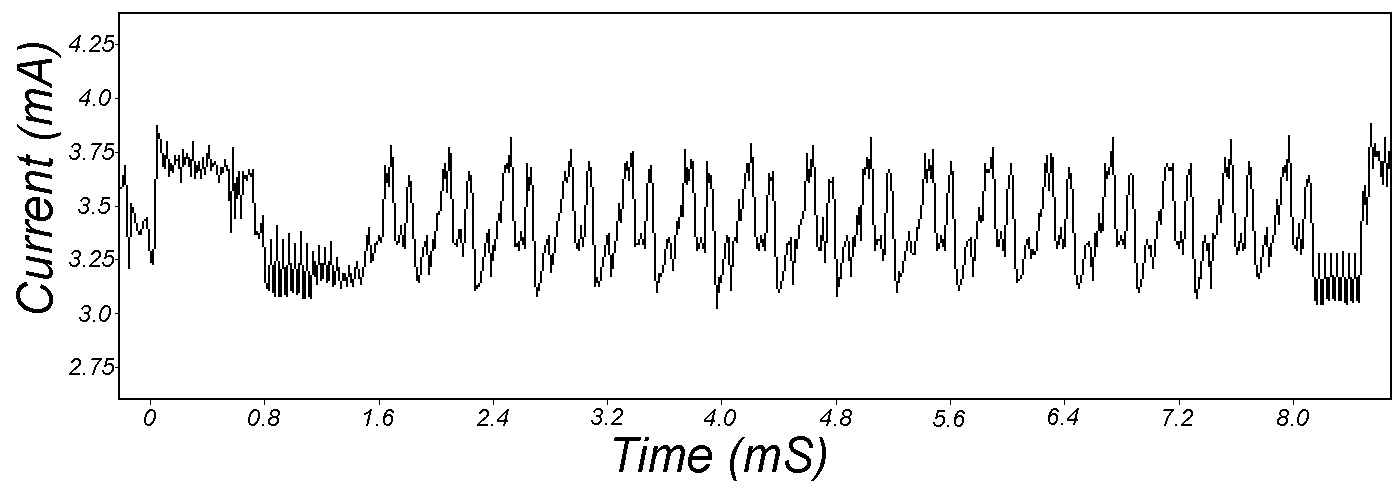
\includegraphics[width=8cm]{des-trace-spa}

	\caption{A trace of the DES algorithm being executed. Credit to Kocher
	et al. \cite{A/Kocher-1999-DPA}.}
	\label{fig:des-trace-spa}
\end{figure}

SPA is simple to implement and execute, and specific operations (such as the
square and multiply operations performed during RSA or individual rounds
performed during AES) can be easily identified, allowing an attacker to easily
deduce what data is being computed. Kocher shows that SPA is effective against
na{\"i}ve implementations of DES, along with other algorithms which do not
contain protections against SPA. Some suggested defences against SPA include:

SPA is best used against simple machines such as smart card readers, which only
perform basic operations. Against more complex machines (such as desktop
computers or FPGAs) however, SPA is not sufficient to perform an attack as it
can be very difficult to identify a single signal from a processor which may be
performing multiple operations in parallel. Additionally, the increased
processing power and additional noise from external process can make sampling
extremely challenging and a single sample will not be enough to recover a
secret. These challenges make implementing a practical attack very difficult in
a realistic scenario.

To counter these issues, Kocher proposes differential power analysis (DPA).
Multiple traces are recorded and these are analysed to guess some secret.
The method suggested by Kocher is as follows \cite{A/Kocher-2011-DPA}:

\begin{enumerate}
	\item{Collect a (usually large) number of traces, including the inputs
		used to produce them.}
	\item{Split the traces into subsets based on their inputs. (Note: this
		is the guessing stage of the attack -- the aim is to find the
		input which has the highest correlation with the power output
		under the assumption the output will be highest when the
		correlation is strongest).}
	\item{For each subset of traces:}
		\begin{enumerate}
			\item{Compute the average trace of the subset.}
		\end{enumerate}
	\item{Compute the difference between the average traces of the subsets
		and note the result.}
		\begin{itemize}
			\item{If the average traces show little to no
				difference then the input value was not in the
				secret.}
			\item{If the average traces show a clear difference
				then the input value was in the secret.}
		\end{itemize}
\end{enumerate}

The rationale here is that if a sufficient number of traces are analysed in
this manner, even miniscule differences between the outputs of the algorithm
can be guessed. A demonstration of DPA is shown in figure
\ref{fig:des-trace-dpa} and the method described above can be used to guess
individual bits used in DES and AES encryption, as shown by Kocher et al.
\cite{A/Kocher-1999-DPA, A/Kocher-2011-DPA}.

\begin{figure}[h]
	\centering

	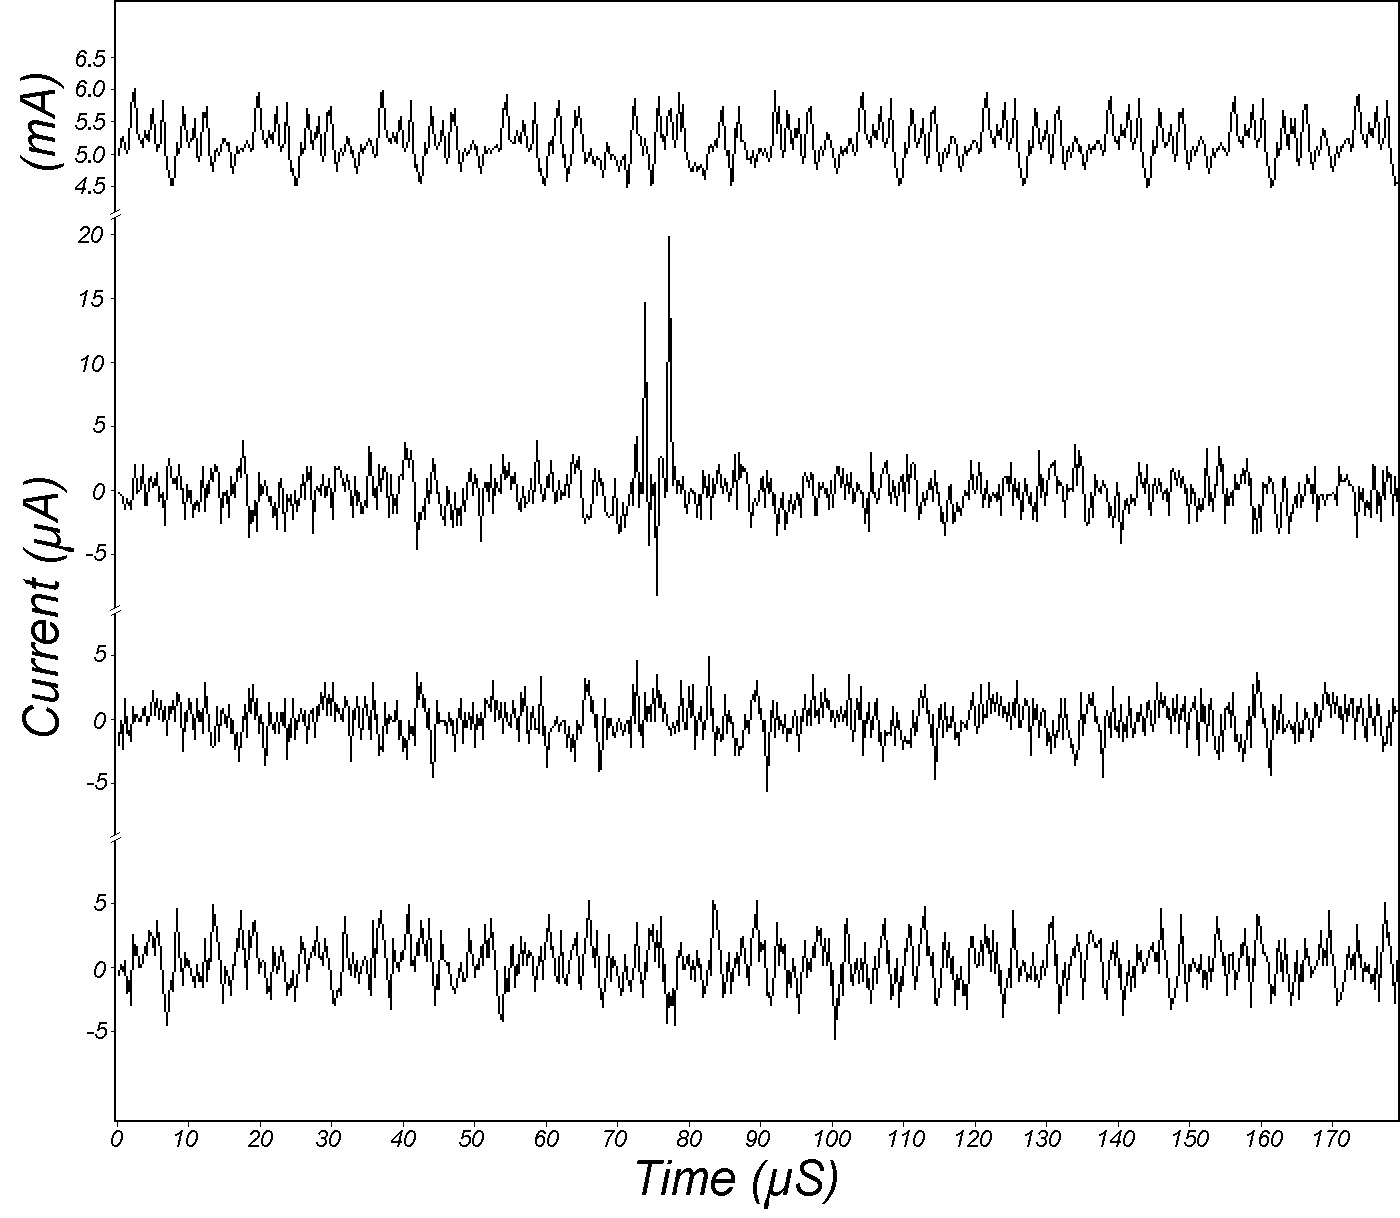
\includegraphics[width=8cm]{des-trace-dpa}

	\caption{Traces showing DPA being executed against DES. The first trace
	is a reference, the second is a correct guess while the last two are
	incorrect guesses. Credit to Kocher et al. \cite{A/Kocher-1999-DPA}.}
	\label{fig:des-trace-dpa}
\end{figure}

Kocher recommends the use of blinding methods again to prevent these sorts of
attacks. Additionally, they also recommend increasing the signal-to-noise
ratio: this can be done either by increasing the amount of noise in a sample so
attacks are more challenging to carry out, or by reducing the level of leakage
using techniques such as balancing. Both of these are highly effective at
creating algorithms that are resistant to DPA.

To combat DPA resistant algorithms and for scenarios where the number of traces
that can be extracted is very limited (e.g. due to physical security measures,
etc.), template attacks were proposed by Chari et al.
\cite{A/Chari-2003-Template}. Here, an adversary uses an identical copy of the
victims device to create a profile of the attack. The attacker uses the device
copy to simulate the attack, creating potentially thousands of power traces
with various keys and plaintexts to produce a ``template". This template can
then be analysed along with a number of traces from the victims device to
complete the attack -- given enough preprocessing, it is possible to recover a
key using just one victim trace. The steps to carry out this attack are
described below:

\begin{enumerate}
	\item{Using the copy of a device, create a large dataset of power
		traces.}
	\item{Create a template of the device by measuring certain points of
		interest during the cryptographic operation.}
	\item{Using the traces from the victims device, apply the template and
		use this to find keys/subkeys. If necessary, repeat till the
		entire secret is recovered.}
\end{enumerate}

The number of victim traces required varies depending on the quality of the
template, which can increase processing times. This attack has the advantage
that only a very small number of traces (potentially just one) are needed to
break a cryptosystem; conversely a large amount of time must be spent setting
up the attack, including creating traces and templates alongside choosing the
appropriate points of interest.

Both DPA and template attacks have been shown to be highly effective at
breaking cryptographic systems, both from their original papers alongside the
research that has stemmed from them. In 1999, Goubin and Patarin demonstrated a
practical DPA attack against DES, and also showed several practical methods
which can be used to increase DPA resistance \cite{A/Goubin-1999-DPA}.
Velegalati et al. showed a DPA attack against AES running on an FPGA system in
2008 \cite{A/Velegalati-2008-DPA}. FPGAs are resistant to SPA attacks given the
amount of noise that they produce -- this paper demonstrates that DPA is able
to counter the noise-to-signal ratio and find the secret. The Trivium and Gain
stream ciphers of the eSTREAM cipher project were shown to be susceptible to
DPA, with Fischer et al. demonstrating a novel technique to remove all the
noise and leave the pure signal \cite{A/Fishcer-2006-DPA}. Attacks against
ECDSA using DPA were shown by Itoh et al. and separately by Wu et al.
illustrating that DPA is effective against elliptic curve cryptography
\cite{A/Itoh-2003-DPA, A/Wu-2009-DPA}. DPA was also shown to be effective
against implementations of RSA, as exemplified by Yen et al.
\cite{A/Yen-2005-DPA}.

In 2004, Oswald and Rechberger published a paper which implemented template
attacks \cite{A/Oswald-2004-Template}. This paper was particularly important as
it covers several additional details vital to ensuring the success of the
attack, including how to preprocess data and how to select points of interest,
which are not covered by Chari et al. and shows that using preprocessing
techniques improves classification by a significant factor. In 2006, Oswald
showed that masking techniques used as a defense mechanism against DPA could be
circumvented using a combination of DPA and template attacks, and showed an
attack against AES encryption \cite{A/Oswald-2007-Template}. An attack on ECDSA
was shown by Medwed in 2008, demonstrating again that elliptic curve
cryptography (which is designed to be resistant to side channel attacks, in
particular timing attacks) is vulnerable to template attacks and power
monitoring side channels \cite{A/Medwed-2008-Template}.

%}}}

% Application of ML to SCAs.
%{{{

\subsection{Application of ML to SCAs}
\label{sec:application-ml-scas}

Previous work has been done to apply machine learning techniques to side
channel attacks. The earliest examples of this date back to 2011, when Hospodar
et al. used Least Squares Support Vector Machines to attack the AES encryption
scheme \cite{A/Hospodar-2011-ML-Template}. It was found that LS-SVMs had a very
high success rate, dependent mostly on the parameters used for the machine
learning technique rather than on the number of traces used for training the
SVM. It was noted that when using an extremely small number of traces (500),
the SVM performed poorly, however this was also true of template attacks. The
paper concludes showing that future work in this area could prove to be highly
fruitful for the future -- while SVMs are heavier compared with standard
template attacks, they could pave the way for alternative machine learning
methods.

In 2015, Lerman et al. revisited the idea of machine learning being used for
template attacks, covering the effectiveness of ML techniques in this area to
date \cite{A/Lerman-2015-ML-Template}. This paper was particularly concerned
with the so-called ``curse of dimensionality": the idea that data with a large
number of features is more difficult to analyse and extract results from
despite seemingly having more detail due to the range of features. Lerman
suggested that while template attacks are theoretically better, ML based
techniques may prove to be more practical. This is reinforced by their earlier
research, where a machine learning approach against AES reduced the number of
traces required to carry out an efficient and correct attack
\cite{A/Lerman-2015-ML-AES}. Future survey work including Picek et al. were
more in favour of machine learning techniques, going so far as to suggest that
traditional methods such as template attacks are no longer sufficient for
identifying security vulnerabilities in systems \cite{A/Picek-2017-ML}.

With the diversity of systems and devices that can be used to perform attacks,
researchers were interested in how machine learning can help alleviate the gap
between different devices. Wang et al. showed that using different devices can
decrease the performance of MLPs used for by up to 75\%, even if identical
chips are used \cite{A/Wang-2019-ML}. To counter this, deep learning models can
be used, as demonstrated by Das et al. who showed that accuracies greater than
99.9\% can be achieved despite multiple devices being used for side channel
attacks \cite{A/Das-2019-DL}. 

A survey paper from 2020 by Hettwer et al. reviewed the current state of the
art with respect to machine learning techniques being applied to side channel
attacks \cite{A/Hettwer-2020-SCAML-Survey}. The main findings were as follows:

\begin{itemize}
	\item{ML can be used to achieve various outcomes depending on the
		scenario, including direct key recovery, recovering
		intermediate key states, mask recovery (which can then be used
		to perform direct key recovery later) and aligning traces.}
	\item{ML techniques can also be used in many parts of the general SCA
		workflow, including preprocessing and feature engineering to
		remove noise and increase success rates.}
	\item{Deep learning techniques enjoy great success but without
		hyperparameters being specified it can be difficult to
		reproduce research.}
\end{itemize}

While the majority of research in this area focuses on supervised learning
techniques used for power analysis side channel attacks, there is a growing
interest ML methods used for timing attacks. A recent paper from Luo et al.
demonstrates a novel reinforcement learning technique used for performing
cache-timing attacks called AutoCAT \cite{A/Luo-2023-AutoCAT}. This method is
unique as it poses the problem of timing attacks as a game where the algorithm
must guess the secret. This approach could prove highly promising in developing
novel algorithms for attacking systems remotely.

Finally, in 2021, researchers at Google published SCAAML: a deep learning
framework used for attacking cryptosystems using side channel attacks
\cite{W/SCAAML, A/Bursztein-2023-DL}. This library can be used to carry out
attacks based around machine learning and encourage further research.

%}}}

%}}}

% Project specification.
%{{{

\section{Project Specification}
\label{sec:project-specification}

This section covers the specification of the project, including experimental
design, success criteria, project contributions, legal/ethical issues, risks
and mitigations, and a timeline of deliverables.

% Aims and Objectives.
%{{{

\subsection{Aims and Objectives}
\label{sec:aims-and-objectives}

The broad aim of this project is to carry out an empirical analysis to compare
SCAs which employ ML techniques with traditional SCA approaches. To achieve
this, a series of experiments around timing and power analysis attacks on the
OpenSSL \cite{W/OpenSSL} implementations of RSA \cite{A/Rivest-1978-RSA} and
ECDSA \cite{A/Johnson-2001-ECDSA} will be performed. The traditional (non-ML)
techniques that will be used are standard timing attacks for the timing side
channel and DPA for the power consumption side channel, on both algorithms. The
ML techniques used will be reinforcement learning for timing attacks and deep
learning for power monitoring attacks. These attacks will then be used to carry
out a series of experiments to evaluate the overall efficacy of ML-based SCAs
(see section \ref{sec:experimental-design} for more details).

The following list specifies the success criteria that the project will be
evaluated against:

\begin{itemize}
	\item{An implementation of a non-ML timing attack against OpenSSL's
		RSA and ECDSA algorithm.}
	\item{An implementation of a non-ML DPA attack against OpenSSL's
		RSA and ECDSA algorithm.}
	\item{An implementation of a ML-based timing attack against OpenSSL's
		RSA and ECDSA algorithm.}
	\item{An implementation of a ML-based power analysis attack against
		OpenSSL's RSA and ECDSA algorithm.}
	\item{A final report describing a series of experiments carried out
		with these attack implementations, including a discussion of
		the results.}
\end{itemize}

For the project to be considered successful, it must complete these success
criteria.

%}}}

% Experimental Design.
%{{{

\subsection{Experimental Design}
\label{sec:experimental-design}

This section describes a series of experiments that will be performed to
understand how machine learning techniques can be used to improve non-ML
techniques with SCAs. The proposed scenario is as follows: some data \( C
\) is signed with some algorithm \( A \) and some private key \( k \) to
produce some signature \( S \): \( A(C, k) = S \). The attacker knows the
data \( C \), the signature \( S \) and the algorithm \( A \) (which is either
RSA or ECDSA), and the objective is to find the secret key \( k \).

To achieve this, the attacker will use timing attacks (similar to Kocher and
Brumley \cite{A/Kocher-1996-Timing, A/Brumley-2011-Remote-TAs,
A/Brumley-2005-Remote-TAs}) and DPA attacks (similar to Kocher
\cite{A/Kocher-1999-DPA}). These will be implemented as part of the project,
and represent the non-ML versions of timing and power monitoring attacks
respectively. Additionally, the attacker will also use machine learning based
SCAs to attack the cryptosystem, specifically reinforcement learning (similar
to Luo et al. \cite{A/Luo-2023-AutoCAT}) and deep learning (similar to SCAAML
\cite{W/SCAAML}). The attacker will then implement these attacks against the
OpenSSL implementations of these attacks using an unknown key and some data of
their choice. Versions of OpenSSL which are vulnerable to these attacks may be
used: the aim is not to discover new attacks, instead it is to compare machine
learning with analytical techniques. To do this, the experiment will measure
the time taken to train the different models, whether or not the model could
successfully carry out an attack, the precision, accuracy, recall and F1 score
of the models and compare this with the number of traces and amount of time
taken to carry out analytical techniques. Finally, the experiment will use
these results to carry out an evaluation of ML techniques compared with
traditional SCA methods.

%}}}

% Project Contributions.
%{{{

\subsection{Project Contributions}

This project contributes to the wide scientific community by performing
comparative empirical analysis of machine learning techniques for side channel
attacks, which has not previously been done before (as shown in section
\ref{sec:literature-review}). While individual analysis have been done when
exploring novel ideas, a study on the effectiveness of ML based SCAs with
traditional SCAs has not been conducted. Are ML techniques well suited to SCA
problems? Can they be used to advance the field and are they practical to
implement? Do they help find vulnerabilities that are not discoverable with
traditional techniques? Are they more effective when compared with traditional
techniques or are there trade-offs to consider? It is these sorts of questions
that the study proposed above will help to answer, and help direct the future
course of this field.

%}}}

% Legal and Ethical Issues.
%{{{

\subsection{Legal and Ethical Issues}
\label{sec:legal-and-ethical}

This project contains no significant legal issues. The algorithms to be worked
with (ECDSA and RSA) and their implementation software (OpenSSL) are publicly
available. The algorithms for RSA and ECDSA are well known to the wider
security community, are not encumbered by patents, and are commonly implemented
in multiple libraries and experimented on by security researchers. The OpenSSL
software implementation is licensed under the permissive Apache 2 licence or
the OpenSSL and SSLeay dual licence depending on the version release. Both of
these licences permit the user to perform scientific experiments on the
software and provide the software ``as is", along with including some terms and
conditions regrading redistribution -- this project will not be redistributing
the OpenSSL software so this is not of concern.

As the project does not process any personal information, there are no ethical
concerns around ensuring privacy. There are some ethical concerns that the
project could be used to discover vulnerabilities in the OpenSSL software or
the RSA/ECDSA algorithms, and that these vulnerabilities could be used in
unethical ways such as to steal secret user information. This is discussed in
more detail in section \ref{sec:risks-and-mitigations}.

%}}}

% Risks and Mitigations.
%{{{

\subsection{Risks and Mitigations}
\label{sec:risks-and-mitigations}

This project is purely a scientific project involving experimentation on open
source software, so there are no environmental, health, safety, privacy or
financial risks. There are no legal risks as the software and algorithms being
used are open source. There are some project and security risks, which are
described in table \ref{tbl:risks-mitigations} along with some mitigation
strategies.

\begin{table}[h]
	\centering
	\footnotesize

	\begin{tabular}{|p{3cm}|l|l|p{9cm}|}
		\hline
		\textbf{Risk} & \textbf{Likelihood} & \textbf{Impact} &
		\textbf{Mitigation} \\
		\hline
		The project could be used for malicious purposes. & Low & High
		& The project will be released under the MIT public license to
		encourage security research around this area and to ensure that
		the playing field is even: both the security community and
		potential malicious actors will have access to the same
		resources. Additionally, the project focuses on vulnerabilities
		which have already been discovered and mitigated. Finally, if
		any new vulnerabilities are discovered, an appropriate and
		ethical disclosure strategy will be followed to be discussed
		with the supervisor as needed. \\
		\hline
		The project may not be completed on time. & Low & High &
		A well defined success criteria specifying the expected
		outcomes of this project has been given in
		\ref{sec:aims-and-objectives} along with a Gantt chart
		specifying when they are expected to be completed in section
		\ref{sec:timeline-of-deliverables}. Additionally, regular
		updates in the form of weekly meetings or emails will be
		provided to the supervisor along with a log that will be
		regularly updated to ensure that progress is tracked and
		followed. \\
		\hline
	\end{tabular}

	\caption{Identified risks and their mitigations.}
	\label{tbl:risks-mitigations}
\end{table}

%}}}

% Timeline of deliverables.
%{{{

\subsection{Timeline of Deliverables}
\label{sec:timeline-of-deliverables}

A Gantt chart describing a timeline of expected tasks is shown in figure
\ref{fig:gantt-chart}.

\begin{figure}[h]
	\centering

	\begin{ganttchart}[x unit=0.8cm,
		y unit title=0.5cm,
		y unit chart=0.5cm,
		vgrid,hgrid,
		title height=1,
		bar height=0.7,
		title label font=\footnotesize,
		bar label font=\footnotesize,
		]{1}{17}
		\gantttitle{Term:Week}{17} \\
		\gantttitle{1:11}{1}
		\gantttitle{1:12}{1}
		\gantttitle{H:1}{1}
		\gantttitle{H:2}{1}
		\gantttitle{H:3}{1}
		\gantttitle{H:4}{1}
		\gantttitle{2:1}{1}
		\gantttitle{2:2}{1}
		\gantttitle{2:3}{1}
		\gantttitle{2:4}{1}
		\gantttitle{2:5}{1}
		\gantttitle{2:6}{1}
		\gantttitle{2:7}{1}
		\gantttitle{2:8}{1}
		\gantttitle{2:9}{1}
		\gantttitle{2:10}{1}
		\gantttitle{2:11}{1} \\
		
		\ganttbar[name=research]{Research}{1}{6} \\
		\ganttbar[name=tas]{Impl. TAs}{4}{8} \\
		\ganttbar[name=dpa]{Impl. DPA}{5}{9} \\
		\ganttbar[name=rl]{Impl. RL (TAs)}{6}{10} \\
		\ganttbar[name=dl]{Impl. DL (PAs)}{6}{10} \\
		\ganttbar[name=experiments]{Experiments}{12}{15} \\
		\ganttbar[name=report]{Final Report}{3}{17}
	
		\ganttlink{research}{tas}
		\ganttlink{research}{dpa}
		\ganttlink{research}{rl}
		\ganttlink{research}{dl}
		\ganttlink{research}{report}
		\ganttlink{tas}{experiments}
		\ganttlink{dpa}{experiments}
		\ganttlink{rl}{experiments}
		\ganttlink{dl}{experiments}
		\ganttlink{experiments}{report}
	\end{ganttchart}
	
	\caption{A Gantt chart showing the timeline of deliverables.}
	\label{fig:gantt-chart}
\end{figure}

The tasks shown in figure \ref{fig:gantt-chart} correlate to the expected
deliverables listed in the success criteria: an implementation of a timing
attack, a DPA attack, a deep learning attack and a reinforcement learning
attack.

%}}}

%}}}

% Epilogue.
%{{{

\pagebreak

\pagenumbering{gobble}

\printbibliography

\end{document}

%}}}
